\documentclass[a4paper]{report}
%Uncomment this for better screen readable report 
%\documentclass[a4paper]{scrreprt}
\usepackage[english]{babel}
\usepackage[pdftex]{graphicx}
\usepackage{acronym}
\usepackage{verbatim}

\usepackage{color}
\definecolor{light-gray}{gray}{0.95}

\usepackage{listings}
\lstset{ %
basicstyle=\footnotesize,       % the size of the fonts that are used for the code
numbers=left,                   % where to put the line-numbers
numberstyle=\footnotesize,      % the size of the fonts that are used for the line-numbers
stepnumber=1,                   % the step between two line-numbers. If it is 1 each line will be numbered
numbersep=5pt,                  % how far the line-numbers are from the code
backgroundcolor=\color{light-gray}, % choose the background color. You must add \usepackage{color}
showspaces=false,               % show spaces adding particular underscores
showstringspaces=false,         % underline spaces within strings
showtabs=false,                 % show tabs within strings adding particular underscores
frame=single,   		% adds a frame around the code
tabsize=4,  	        	% sets default tabsize to 2 spaces
captionpos=b,   		% sets the caption-position to bottom
breaklines=true,    	        % sets automatic line breaking
breakatwhitespace=false,        % sets if automatic breaks should only happen at whitespace
escapeinside={\%}{)}            % if you want to add a comment within your code
}

\usepackage[a4paper=true,pagebackref=true]{hyperref}
\hypersetup{
	colorlinks,%
	citecolor=black,%
	filecolor=black,%
	linkcolor=black,%
	urlcolor=black
}
\title{ESSIG - \acl{ESSIG}}
\author{
	Ewoud Kohl van Wijngaarden (ewoud@kohlvanwijngaarden.nl) \\
	\and
	Wilfried van Asten (w.g.g.vanasten@student.utwente.nl)\\
	\and
	Ruud Harmsen (r.harmsen@student.utwente.nl)\\
	\and
	Mark Florisson (markflorisson88@gmail.com)
	\\
	\\
	\small Ontwerpproject (192199109) \\
	\small University of Twente \\
	\small Faculty of Electrical Engineering, Mathematics and Computer Science
}
\date{}

\begin{document}
\maketitle

\setcounter{tocdepth}{10}
\renewcommand\contentsname{Table of Contents}
\newcommand{\UC}{
	$\mu$C  
}

\tableofcontents
\clearpage\selectlanguage{english}

\begin{block}{\large \smash{Introduction}\vphantom{Introduction}}
\end{block}


\chapter{Related work}
There are countless simulators available for various embedded architectures.
However, there do not appear to be many simulator generators around. The only
other project that we have been able to find is CGEN, which stands for
Cpu tools GENerator. It can generate simulators, assemblers and disassemblers. 
The generator is implemented in Scheme, which is also the
language used to write the specification of the Instruction Set Architecture,
"inspired by GCC's RTL and by the Scheme programming language, theoretically
taking the best of both" \cite{CGEN}.\\
Currently the opcodes table and an ISA level simulator need to be specified, 
but the goal is to have "an application independent description of the CPU".\\
The documentation claims good speed by implemented a threaded interpreter with
the use of computed gotos, where "about three host instructions per target
instruction" are needed to jump to the next instruction handler. A typical
instruction handler takes about ten host instructions.\\
\\
CGEN is used in some other projects, such as SID and GDB. SID is a "framework
for building computer system simulations" \cite{SID}. GDB is the GNU DeBugger,
which can be used to debug a variety of languages on a lot of target
platforms \cite{GDB}. Currently several of
simulators provided by GDB use CGEN. "These simulators use
a combination of the CGEN-generated files, common files in the sim/common
directory of GDB releases, and custom target-specific code". This
functionality can be used by issuing 
\texttt{target \textless sim\textgreater} from the GDB command
line (if built with \texttt{--enable-sim}), after which programs can be loaded
and run in the usual manner.

\chapter{Overview}
\ac{ESSIG} is roughly composed out of three components. First we have
the input language, which can be used to describe the micro controller a
simulator should be generated for. Than we have a generator, which
creates an implementation of the private API (see VM) that the VM can
use in simulating the micro controller. Than we have our VM, in which
the micro controller will be simulated. It exposes a public API to a
client which can then simulate programs like they were running on the
simulator. The following diagram illustrates how the components relate
to each other.

\begin{center}
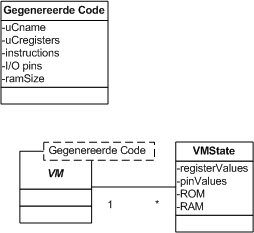
\includegraphics[width=5.376cm,height=4.932cm]{Essig-img002.png}
\end{center}


\chapter{AVR Microcontroller}
For this project, the AVR \ac{UC} is chosen as a base for the \ac{ESSIG}. This
is because the AVR instruction set has simple instructions. For every \ac{UC}
available (e.g. AVR, PIC), there is a specification available. This is often a
PDF file which describes the \ac{UC} in a semi-formal way, which makes it hard
to parse.

Because of this a new specification language had to be created. We chose to
define a new language instead of reusing an existing one because the
description should be easy to write, readable, flexible but also powerful, 
and we knew of no
existing language for this specific purpose that met all those requirements. 
The goal of this new language is to formally describe the entire \ac{UC}s 
specification and make it easy to parse. With this specification a simulator 
can be generated. Thus creating a simulator for a \ac{UC} should be as easy 
as writing a specification for that microcontroller.

\chapter{Grammar}

\section{The Grammar}
The grammar consists of 4 sections. These sections are:
\begin{enumerate}
\item Parameters
\item Registers
\item Maps
\item Instructions
\end{enumerate}

\subsection{Parameters}
In this section all parameters of a \UC are specified. Parameters are: 


\begin{itemize}
\item number of \ac{GPRS} 
\item endianness
\item standard clock cycles needed for 1 instruction (can be overridden per instruction)
\item opcode size (AVR uses 16 bit opcodes, PIC uses 14 bit opcodes).
\end{itemize} 

\subsection{Registers}
In this section the offsets of register values are specified. Currently a little hack is used to address bits in the \ac{SREG}.

\subsection{Maps}
A \ac{UC} has several ranges of addresses. These can be specified below. These address ranges are:
\begin{itemize}
\item chunk = The whole block of memory used for the microcontroller (all other ranges need be addressed in this chunk).
\item register = The location of the \ac{GPRS}.
\item io = The input and output ports of the microcontroller.
\item ram = The \ac{RAM} address range, this is memory that can be used by the user program.
\item rom = The \ac{ROM} address range, the user code is stored in here. 
\item print = This is a custom range used for outputting information in the command line information of the simulator. If in the simulator a value is written to an address in this range, the simulator will print this value.
\end{itemize}

\subsection{Instructions}
The biggest part of the grammar, the instructions. Each instruction needs an opcode. For usage of these instructions, check the user guide.

\section{Design choices and problems}
The biggest problem encountered was that we started to fast on the grammar. We just took the \ac{UC} and started away, but we should have read the whole specification beforehand. This would have saved a lot of time during the writing of the grammar.

\subsection{Opcodes}
We chose to parse the opcodes, not in the ANTLR language, but in inline Java code. This is done because we found it much easier to do in Java.

\section{Future of the grammar}
Things that have to be done to complete the grammar are:
\begin{itemize}
\item Check compatibility of the grammar with other {\UC}'s than the ATMEL AVR.
\item Add support for floating point numbers.
\item In the section 'parameters' the size of a register should be added, e.g. "register-size = 8;" which are 8 bits.
\item The section 'registers'
\begin{itemize}
\item This section should be renamed to a better suitable name such as 'offsets'.
\item Declaration of single BIT's should be possible. The bits in the \ac{SREG} are now set with a little java hack in the code, it checks if the IDENTIFIER is one of these "CZNVSHTI".  
\item Size of an offset should be declareable.
\end{itemize}
\item Declaration of \ac{UC} peripherals like USART, SPI, I2C, ADC.
\end{itemize}

\chapter{Simulator}
The final simulator is composed of two components: A general VM and a
simulator which is generated. The VM contains things common to all 
microcontrollers and supplies debug functionality. The simulator is generated from a description file. Communication between the VM and the generated simulator is accomplished 
by calling functions directly with the current state of the simulation. The following
subsections describe each component in detail.

\section{VM}

The VM is a library in which functions are gathered that most simulators
have in common. These functions are defined in terms of a private API
for which implementations can be generated using the generator and the
definition language. Linked together they form a library that can run
programs like they were running on the simulated microcontroller. It
is state driven in that most functions are parameterised with a state
which is then manipulated to the desired state by the function. This
design gives the client the freedom to manipulate and read the
state, which when used properly gives interesting possibilities when
debugging a program. The interpreter can keep a list of differences of the
state so program execution can be reversed at any time to a desired point,
after which the user may modify the state manually from the debugger after
which execution can be resumed with a modified state.

\section{Micro Controller state}
To be able to let the VM execute any code for any microcontroller we
defined a structure that could represent any microcontroller state. It
has all things that all microcontrollers have in common, namely a RAM space, a
ROM space, a register file and an I/O space.
Our specification has all information needed
to generate this state and that is exactly what the VM does. It uses the
description compiled into the simulator part and creates an initial state for 
a simulation. This state is
then passed to every function that needs it to operate, which means that the 
VM can for example manage and run several programs simultaneously (although
the debugger fontend does not currently support multiple simultaneous
simulations). \\
In addition to a simulation state, the user may also decide to keep track of
differences in the state, which is managed by a separate stack of diffs.
These diffs can be used to backtrack the program execution. This relatively loose structure gives
a lot of interesting capabilities to the client (e.g. save the diffs
and state to the disk and resume exectution later on (with
full backtracking)).

\section{The Generated Simulator}
The generated simulator exposes a private API which contains the
implementations that simulate the instructions, the information 
for the VM to allocate an appropriate simulation state and the information 
to disassemble the target instruction set into a representation that allows 
efficient lookup. The opcode specification is stored in small 
structures, each of which contains a pointer to the associated instruction 
handler, the name of the opcode, the bits that constitute the opcode and a 
bitmask that can be applied to an instruction in order to obtain the 
associated opcode. The
instruction handlers are private functions of the generated simulator,
but they all have the same signature as declared by the VM. During program
execution (i.e., during simulation), the VM passes execution to these handlers
whenever an instruction needs to be executed. These handlers then manipulate
the state through functions exposed by the VM.

\section{The Debugger}
The debugger frontend provides the user with a debugger that can control and
inspect the simulation. Breakpoints may be set for symbol names or addresses,
programs may be simulated (multiple times) and whenever execution is halted
(or even after the program has terminated) the simulation state may be inspected and
altered and execution may be reversed. The frontend uses the readline library
(indirectly) to provide command line editing and history.

\section[Interrupt Handling]{Interrupt Handling}
\begin{comment}
Interrupts in \ac{ESSIG} can occur at two different levels:

\begin{enumerate}
\item {
From outside of the VM through the vm\_interrupt method }
\item {
From a peripheral }
\end{enumerate}
\end{comment}
Interrupts may be specified by callbacks that can be registered with the VM
(with the \texttt{vm\_register\_interrupt\_callable} function). When the debugger
is used, plugins may be written in Python and put into the \texttt{vm/plugins}
directory.\\
Each simulation may have a policy that can govern whether or not the interrupt will be
passed on to the simulator. When interrupts should be handled, a user-supplied
\texttt{set\_interrupt} method will be called every step with the state of the
simulation and a (potentially NULL) diff pointer. The set\_interrupt function
should then inspect \texttt{state->interrupts} and modify the state of the
microcontroller appropriately. A subsequent \texttt{handle\_interrupt}
function (with a signature equivalent to \texttt{set\_interrupt}) is 
called every step to check the simulation state for an
interrupt flag. Based on the intricacies of the microcontroller, this function
should then modify
the passed-in state accordingly. This may mean pushing the program counter on the stack, 
changing
the stack pointer and writing the address of the interrupt handler specified
in the debuggee to the program counter.

After all this the VM resumes execution with the potentially modified state.
It is up to the implementor of \texttt{set\_interrupt} and 
\texttt{handle\_interrupt} to use the functions of the VM to modify the state.
If those functions are used along with a diff stack, changes will be
registered in the diffs. If the state is modified without using any VM
function,
changes will not registered in the diffs and hence reverse-stepping will be oblivious to
any changes incurred by an interrupt handler. This means code could be executed
once with an interrupt handler and once without, and changes in state or
control flow may be observed.

\section[Opcode parsing]{Opcode parsing}
In any simulator at some point opcodes will have to be parsed in order
to determine what code to execute. There are a lot of different
solutions to this problem and we will discuss a few of them here and
after that explain the solution we chose.

\subsection[Switch statement]{Switch statement}
To a lot of simulators out there this is the preferred method. The idea
is that you input the opcode or a part of the opcode into a switch
statement and continue execution at the matched case. This method has
one disadvantage: The case statement can't be generalized to any
simulator since the opcodes are (or can be) very different accross
different architectures, unless the instructions are disassembled first and the
switch is on the disassembled opcodes (or some other associated unique key) instead.

\subsection{Some sort of function array}
This isn't used that much at all but for smaller architectures it can be
done. The idea is that you have an array of functions that handle an
opcode and that you index the array using the opcode. But as mentioned
for architectures with a relatively large opcode this array would
become far too large and since some instructions have some argument(s)
embedded in the opcode a lot of functions appear multiple times in the array.

\subsection{Our solution}
We wanted to be able to find our instruction in an array efficiently without
having to keep entries for every possible opcode. So instead we list the
opcode with variable parts masked to zero, and a bitmask that can be applied
to an instruction to obtain the associated opcode. These opcodes and masks are
specified in the microcontroller description file. Before execution starts,
all the instructions are disassembled, which means that each instruction holds
a key from which an instruction handler can be obtained in constant time. This gives the advantage of fast opcode resolution in exchange for a slightly longer load time. 


% TODO: This idea is further illustrated in the following diagram:

\section[PC incrementation]{PC incrementation}
In different microcontrollers the program counter either points to the
current instruction or the next instruction. Because we delegate
program counter incrementation to our instruction handlers, both
situations can be emulated quite easily by either incrementing the
program counter at the beginning of the instruction handler (to
indicate the next instruction) or at the end of the handler.

To illustrate this consider the following two pseudo code
implementations of rcall:

\lstset{caption=PC points to next instruction}
\begin{lstlisting}
PC = PC + 1
PUSH PC
PC = PC + k
\end{lstlisting}

\lstset{caption=PC points to current instruction}
\begin{lstlisting}
PUSH (PC + 1)
PC = PC + k
PC = PC + 1
\end{lstlisting}

It can be seen that in a microcontroller in which the PC points to the
next instruction the push operation is simpler.

In the above example the effects of the instruction was exactly the same
but in microcontrollers in which it is possible to push the PC (This
is not so in atmel microcontrollers) there can be a difference:

\lstset{caption=PC points to next instruction}
\begin{lstlisting}
PC = PC + 1
STORE PC on stack
\end{lstlisting}

\lstset{caption=PC points to current instruction}
\begin{lstlisting}
STORE PC on stack
PC = PC + 1
\end{lstlisting}

Now in the first the top of the stack is the address of the next
instruction but in the second the address of the current instruction.
It also illustrates that our language can handle both situations
because the incrementation of the PC is handled by the instruction
handler.

\chapter{User guide}
This chapter describes how to use \ac{ESSIG}.

\chapter{Limitations and future work}
Dit verslag beschrijft de bedachte programmeertaal Expr en beschrijft de
ontwikkeling van de bijbehorende compiler.

Aan het eind van het verslag zijn enkele appendices opgenomen. 


\bibliographystyle{plain}
\clearpage
\addcontentsline{toc}{chapter}{Bibliography}
\bibliography{Essig}

\appendix
\chapter[Grammar explanation]{Microcontroller specification language}
Op het laatste moment hebben we besloten om de ANTLR specificaties niet
uit te printen, test, test, test.

\chapter[Evaluation]{Evaluation}
De code en voorbeeldin- en uitvoer van een uitgebreid Expr programma is
\cite{atmelISA} opgenomen in deze appendix.

\chapter{Acronyms}
\begin{acronym}
 \acro{ESSIG}{Embedded Systems SImulator Generator}
 \acro{UC}{microcontroller}
 \acro{GPRS}{General Purpose RegisterS}
 \acro{SREG}{Status REGister}
 \acro{RAM}{Random Access Memory}
 \acro{ROM}{Read Only Memory}
 \acro{SP}{Stack Pointer}
 \acro{ALU}{Arithmetic Logic Unit}
\end{acronym}

\end{document}
